%%%%%%%%%%%%%%%%%%%%%%%%%%%%%%%%%%%%%%%%%%%%%%%%%%%%%%%%%%%%%%%%%%%%%%%%%%%%%%%%
%2345678901234567890123456789012345678901234567890123456789012345678901234567890
%        1         2         3         4         5         6         7         8

\documentclass[letterpaper, 10 pt, conference]{ieeeconf}  % Comment this line out if you need a4paper

%\documentclass[a4paper, 10pt, conference]{ieeeconf}      % Use this line for a4 paper
\IEEEoverridecommandlockouts                              % This commfreaand is only needed if 
                                                          % you want to use the \thanks command

\overrideIEEEmargins                                      % Needed to meet printer requirements.

\usepackage{color}
\usepackage{graphicx}

\usepackage{amsmath,amssymb,amsfonts,mathrsfs}
\usepackage[colorlinks=true, allcolors=blue]{hyperref}
\usepackage[caption=false,font=footnotesize,labelfont=sf,textfont=sf]{subfig}
\usepackage{stfloats}
\usepackage{algorithm}
\usepackage{algorithmic}
\usepackage{pgf}
\usepackage{tikz}

\DeclareMathOperator*{\argmax}{arg\,max}
\newtheorem{definition}{Definition}

\usetikzlibrary{arrows,automata,calc,petri}
\usetikzlibrary{shapes.multipart}
\usetikzlibrary{shapes.misc}
\tikzset{automatonFig/.style={->,>=stealth',shorten >=1pt,auto,node distance=1.7cm,
                    thick,initial text={}}}
\tikzset{forbidding cross/.style={cross out,draw,-,
         minimum size=0.8cm,thin}}  


%In case you encounter the following error:
%Error 1010 The PDF file may be corrupt (unable to open PDF file) OR
%Error 1000 An error occurred while parsing a contents stream. Unable to analyze the PDF file.
%This is a known problem with pdfLaTeX conversion filter. The file cannot be opened with acrobat reader
%Please use one of the alternatives below to circumvent this error by uncommenting one or the other
%\pdfobjcompresslevel=0
%\pdfminorversion=4

% See the \addtolength command later in the file to balance the column lengths
% on the last page of the document

% The following packages can be found on http:\\www.ctan.org
%\usepackage{graphics} % for pdf, bitmapped graphics files
%\usepackage{epsfig} % for postscript graphics files
%\usepackage{mathptmx} % assumes new font selection scheme installed
%\usepackage{times} % assumes new font selection scheme installed
%\usepackage{amsmath} % assumes amsmath package installed
%\usepackage{amssymb}  % assumes amsmath package installed

\newenvironment{note}
    {
        \color{blue}
    }
    { 
        \color{black}
    }

\title{\LARGE \bf
Hazard Analysis of Human-Robot Systems: An Adversarial Approach based on Supervisor Synthesis and Simulation
}%% this is a working title, we can change it later
%% Alternative title idea: "Risk vs. Realism: Multi-Objective Safety Falsification in the Context of Human-Robot Collaboration"

\author{Tom P. Huck$^{1}$%, Constantin Cronrath$^{1}$, Yuavarj Selvaraj, Christoph Ledermann$^{2}$,\\ Torsten Kröger$^{2}$~\IEEEmembership{Senior Member,~IEEE}, and Bengt Lennartson$^{1}$,~\IEEEmembership{Fellow,~IEEE}% <-this % stops a space
\thanks{*This work was supported
%by Vinnova under the ITEA3 ``AITOC'' (\url{www.itea4.org/project/aitoc.html}) project and by 
the German Federal Ministry for Economic Affairs and Climate Action under the project ``SDM4FZI'' (\url{www.sdm4fzi.de}). The support is gratefully acknowledged.}% <-this % stops a space
% \thanks{$^{1}$Division of Systems and Control, Department of Electrical Engineering, Chalmers University of Technology, Gothenburg, Sweden.
% {\tt\small cronrath@chalmers.se}}%
\thanks{$^{1}$Intelligent Process Automation and Robotics Lab, Institute of Anthropomatics and Robotics (IAR-IPR), Karlsruhe Institute of Technology, Germany.
{\tt\small tom.huck@kit.edu}}%
}


\begin{document}



\maketitle
\thispagestyle{empty}
\pagestyle{empty}


%%%%%%%%%%%%%%%%%%%%%%%%%%%%%%%%%%%%%%%%%%%%%%%%%%%%%%%%%%%%%%%%%%%%%%%%%%%%%%%%
\begin{abstract}
Lorem ipsum dolor sit amet, consectetur adipiscing elit, sed do eiusmod tempor incididunt ut labore et dolore magna aliqua. Ut enim ad minim veniam, quis nostrud exercitation ullamco laboris nisi ut aliquip ex ea commodo consequat. Duis aute irure dolor in reprehenderit in voluptate velit esse cillum dolore eu fugiat nulla pariatur. Excepteur sint occaecat cupidatat non proident, sunt in culpa qui officia deserunt mollit anim id est laborum. Lorem ipsum dolor sit amet, consectetur adipiscing elit, sed do eiusmod tempor incididunt ut labore et dolore magna aliqua. Ut enim ad minim veniam, quis nostrud exercitation ullamco laboris nisi ut aliquip ex ea commodo consequat. Duis aute irure dolor in reprehenderit in voluptate velit esse cillum dolore eu fugiat nulla pariatur. Excepteur sint occaecat cupidatat non proident, sunt in culpa qui officia deserunt mollit anim id est laborum
\end{abstract}

%%%%%%%%%%%%%%%%%%%%%%%%%%%%%%%%%%%%%%%%%%%%%%%%%%%%%%%%%%%%%%%%%%%%%%%%%%%%%%%%
\section{INTRODUCTION}
\label{sec:introduction}
Human-robot collaboration will play an important role in many areas of robotics in the future. Since close physical interactions between humans and robots can lead to hazardous situations, it is vital that the development of human-robot systems is accompanied by a thorough hazard analysis. %For analysis of safety-critical technology, there is already a wide range of methods available, ranging from human expert reasoning over various testing methods to formal verification. 
However, analyzing hazards of HRC systems prior to commissioning is challenging. Due to close interactions and shared workflows, the human becomes a crucial safety-critical system component. While there are numerous methods to assess safety and reliability of the \textit{technical} system components, assessing the effect of the human component is yet an unsolved problem, mainly due to the possibility of unforeseen or erroneous human behavior, which is difficult to foresee.
The traditional approach when considering the impact of human behavior in hazard analyses is to make a-priori assumptions based on expert judgement. Safety standards such as ISO 12100 require that experts define a range of behaviors, including intended use and foreseeable misuse of systems, before conducting a hazard analysis. This approach is generally accepted today. Yet, as the complexity of collaborative tasks and systems continues to grow, it is becoming increasingly difficult for safety engineers to foresee what behaviors may lead to hazardous situations. If critical human behaviors are not considered in the hazard analysis of the overall human-robot system, necessary safeguards may not be implemented, or faults in the safety concept may not be identified. This leads to costly changes at later development stages and, in the worst case, accidents causing human harm.

This paper presents a model-based approach to the hazard analysis of human-robot systems. Rather than making a-priori assumptions about which behaviors are to be expected from the human, this approach treats the human as an adversarial agent who actively attempts to transfer the system into unsafe states. In doing so, the agent provides valuable examples showing how the system's safety measures can fail. This reduces the possibility of critical behaviors being overlooked.

Our approach breaks down the human-robot system into two subsystems representing human and robot, respectively. Both subsystems are modeled on two abstraction levels: Automata models capture the subsystem's interaction on an abstract level, while 3D simulation models capture the physical aspects of the interaction (e.g. sensor detection or collisions). Hazardous behaviors are synthesized automatically from the automata models on the basis of supervisory control theory. The synthesized behaviors are then simulated in a 3D simulation environment to evaluate physical safety aspects which are not sufficiently captured in the automata models.

\section{PRELIMINARIES}
\label{sec:preliminaries}
\subsection{Safety, Hazards and Hazard Analysis}
Lorem ipsum dolor sit amet, consectetur adipiscing elit, sed do eiusmod tempor incididunt ut labore et dolore magna aliqua. Ut enim ad minim veniam, quis nostrud exercitation ullamco laboris nisi ut aliquip ex ea commodo consequat. Duis aute irure dolor in reprehenderit in voluptate velit esse cillum dolore eu fugiat nulla pariatur. Excepteur sint occaecat cupidatat non proident, sunt in culpa qui officia deserunt mollit anim id est laborum. Lorem ipsum dolor sit amet, consectetur adipiscing elit, sed do eiusmod tempor incididunt ut labore et dolore magna aliqua. Ut enim ad minim veniam, quis nostrud exercitation ullamco laboris nisi ut aliquip ex ea commodo consequat. 

\subsection{Extended Finite State Automata (EFSA)}
Lorem ipsum dolor sit amet, consectetur adipiscing elit, sed do eiusmod tempor incididunt ut labore et dolore magna aliqua. Ut enim ad minim veniam, quis nostrud exercitation ullamco laboris nisi ut aliquip ex ea commodo consequat. Duis aute irure dolor in reprehenderit in voluptate velit esse cillum dolore eu fugiat nulla pariatur. Excepteur sint occaecat cupidatat non proident, sunt in culpa qui officia deserunt mollit anim id est laborum. Lorem ipsum dolor sit amet, consectetur adipiscing elit, sed do eiusmod tempor incididunt ut labore et dolore magna aliqua. Ut enim ad minim veniam, quis nostrud exercitation ullamco laboris nisi ut aliquip ex ea commodo consequat. 

\subsection{Supervisory Control Theory}
Lorem ipsum dolor sit amet, consectetur adipiscing elit, sed do eiusmod tempor incididunt ut labore et dolore magna aliqua. Ut enim ad minim veniam, quis nostrud exercitation ullamco laboris nisi ut aliquip ex ea commodo consequat. Duis aute irure dolor in reprehenderit in voluptate velit esse cillum dolore eu fugiat nulla pariatur. Excepteur sint occaecat cupidatat non proident, sunt in culpa qui officia deserunt mollit anim id est laborum. Lorem ipsum dolor sit amet, consectetur adipiscing elit, sed do eiusmod tempor incididunt ut labore et dolore magna aliqua. Ut enim ad minim veniam, quis nostrud exercitation ullamco laboris nisi ut aliquip ex ea commodo consequat. 

\section{RELATED WORK}
% \subsection{Intuitive and Semi-formal Hazard Analysis}
Lorem ipsum dolor sit amet, consectetur adipiscing elit, sed do eiusmod tempor incididunt ut labore et dolore magna aliqua. Ut enim ad minim veniam, quis nostrud exercitation ullamco laboris nisi ut aliquip ex ea commodo consequat. Duis aute irure dolor in reprehenderit in voluptate velit esse cillum dolore eu fugiat nulla pariatur. Excepteur sint occaecat cupidatat non proident, sunt in culpa qui officia deserunt mollit anim id est laborum. Lorem ipsum dolor sit amet, consectetur adipiscing elit, sed do eiusmod tempor incididunt ut labore et dolore magna aliqua. Ut enim ad minim veniam, quis nostrud exercitation ullamco laboris nisi ut aliquip ex ea commodo consequat. 

% \subsection{Simulation-based Hazard Analysis}
Lorem ipsum dolor sit amet, consectetur adipiscing elit, sed do eiusmod tempor incididunt ut labore et dolore magna aliqua. Ut enim ad minim veniam, quis nostrud exercitation ullamco laboris nisi ut aliquip ex ea commodo consequat. Duis aute irure dolor in reprehenderit in voluptate velit esse cillum dolore eu fugiat nulla pariatur. Excepteur sint occaecat cupidatat non proident, sunt in culpa qui officia deserunt mollit anim id est laborum. Lorem ipsum dolor sit amet, consectetur adipiscing elit, sed do eiusmod tempor incididunt ut labore et dolore magna aliqua. Ut enim ad minim veniam, quis nostrud exercitation ullamco laboris nisi ut aliquip ex ea commodo consequat. 

Lorem ipsum dolor sit amet, consectetur adipiscing elit, sed do eiusmod tempor incididunt ut labore et dolore magna aliqua. Ut enim ad minim veniam, quis nostrud exercitation ullamco laboris nisi ut aliquip ex ea commodo consequat. Duis aute irure dolor in reprehenderit in voluptate velit esse cillum dolore eu fugiat nulla pariatur. Excepteur sint occaecat cupidatat non proident, sunt in culpa qui officia deserunt mollit anim id est laborum. Lorem ipsum dolor sit amet, consectetur adipiscing elit, sed do eiusmod tempor incididunt ut labore et dolore magna aliqua. Ut enim ad minim veniam, quis nostrud exercitation ullamco laboris nisi ut aliquip ex ea commodo consequat. 

% \subsection{Formal Verification}
Lorem ipsum dolor sit amet, consectetur adipiscing elit, sed do eiusmod tempor incididunt ut labore et dolore magna aliqua. Ut enim ad minim veniam, quis nostrud exercitation ullamco laboris nisi ut aliquip ex ea commodo consequat. Duis aute irure dolor in reprehenderit in voluptate velit esse cillum dolore eu fugiat nulla pariatur. Excepteur sint occaecat cupidatat non proident, sunt in culpa qui officia deserunt mollit anim id est laborum. Lorem ipsum dolor sit amet, consectetur adipiscing elit, sed do eiusmod tempor incididunt ut labore et dolore magna aliqua. Ut enim ad minim veniam, quis nostrud exercitation ullamco laboris nisi ut aliquip ex ea commodo consequat. 

% \subsection{Combined Approaches}
% Lorem ipsum dolor sit amet, consectetur adipiscing elit, sed do eiusmod tempor incididunt ut labore et dolore magna aliqua. Ut enim ad minim veniam, quis nostrud exercitation ullamco laboris nisi ut aliquip ex ea commodo consequat. Duis aute irure dolor in reprehenderit in voluptate velit esse cillum dolore eu fugiat nulla pariatur. Excepteur sint occaecat cupidatat non proident, sunt in culpa qui officia deserunt mollit anim id est laborum. Lorem ipsum dolor sit amet, consectetur adipiscing elit, sed do eiusmod tempor incididunt ut labore et dolore magna aliqua. Ut enim ad minim veniam, quis nostrud exercitation ullamco laboris nisi ut aliquip ex ea commodo consequat.

\section{OBJECTIVES, ASSUMPTIONS, AND PROBLEM DEFINITION}
% This section formalizes the the hazard analysis problem for human-robot systems and states the underlying assumptions.
As discussed in section \ref{sec:preliminaries}, hazard analysis methods vary in terms of their methodology and the types of hazards they aim to identify. Hazards arising from random failures are \textit{not} considered here. The justification for this omission is that there are already well-established methods to deal with random failures, and state-of-the art safety rated technology achieves extremely low failure rates (e.g., the safety integrity level SIL2, which is commonly used in safety critical robot applications, targets $10^{-7}$ to $10^{-6}$ dangerous failures per hour \cite{STD_IEC61508}). Instead, this paper focuses on systematic hazards, that is, hazards which arise in the interaction between human and robot due to flaws in the design of the system or its safeguards. Our approach to identify such hazards is based on the following assumptions:
\begin{itemize}
    \item[(1)] The system is described by two interacting subsystem models $\mathcal{H}$ and $\mathcal{R}$, with the former representing the human and the latter representing all non-human system components (i.e., robot, sensors, etc.). For brevity, the latter shall simply be called "robot system". The joint human-robot system shall be denoted by $\mathcal{H} || \mathcal{R}$. Concrete modeling formalisms will be introduced in Section \ref{sec:solution}. For now, it is sufficient to assume that each model has a state space and and initial state.
    \item[(2)] The behavior of $\mathcal{H}$ described by sequences of discrete actions from an action space $A_\mathcal{H}$. The set of possible sequences shall be denoted by $\mathcal{L}(A_\mathcal{H})$. For any given human behavior, the robot system reacts in a deterministic manner, which is encoded in $\mathcal{R}$. Hence, the behavior of the human can be regarded as the sole system input on which the behavior of $\mathcal{H} || \mathcal{R}$ depends.
    \item[(3)] There is a user-defined safety specification which maps each system state to a binary value indicating if the state is safe:
    \begin{equation}\mathcal{{SP}}: S_{\mathcal{H} || \mathcal{R}} \rightarrow \{true,false\}\end{equation}
    where $S_{\mathcal{H} || \mathcal{R}}$ is the state-space of $\mathcal{H} || \mathcal{R}$. For the system to be safe, $\mathcal{SP}$ must hold $true$ at all times during the interaction. The system is said to contain a hazard if there exists at least one state in $S_{\mathcal{H} || \mathcal{R}}$ which is (i) unsafe according to $\mathcal{SP}$ and (ii) reachable during interaction. (Note that even the state space of safe systems may contain unsafe states, however, in safe system, these states should not be reachable because the system has appropriate safeguards implemented).
\end{itemize}
Although these assumptions place certain limits on the methodology, we argue that they are justified in many practical cases. A discussion about this can be found in Section \ref{sec:discussion}. For now, we take the assumptions as given and focus on their implications for the hazard analysis problem.

Observe that since the behavior of the human-robot system depends on the human behavior (assumption (2)), the model $S_{\mathcal{H} || \mathcal{R}}$ can be regarded as a function that returns resulting state trajectory $\underline{s}=(s_0, s_1, s_2, ...), s_i \in S_{\mathcal{H} || \mathcal{R}}$ for any given human action sequence $\underline{a} \in \mathcal{L}(A_\mathcal{H})$:

\begin{equation}
    \mathcal{H} || \mathcal{R}: \mathcal{L}(A_\mathcal{H}) \rightarrow S_{\mathcal{H} || \mathcal{R}}^{*}
\end{equation}

If the system contains hazards, there must therefore be at least one action sequence that transfers $S_{\mathcal{H} || \mathcal{R}}$ from the initial state to an unsafe state (assumption (3)).

We can therefore formalize the hazard analysis problem as a \textit{search problem}: Given a model of the human $\mathcal{H}$, a model of the robot system $\mathcal{R}$, and a safety specification $\mathcal{SP}$, we search for action sequences $\underline{a} \in \mathcal{L}(A_\mathcal{H})$, for which the resulting state trajectory $\underline{s}=(\mathcal{H} || \mathcal{R}) (\underline{a})$ contains at least one state unsafe state according to $\mathcal{SP}$.

Framing the hazard analysis in this way is an \textit{adversarial} approach, since we deliberately aim to find human behaviors that lead to unsafe states. As discussed in Section \ref{sec:introduction}, this is a significant difference to traditional hazard analysis methods which generally pre-define a certain range of expected human behaviors.

\section{PROPOSED SOLUTION}
\label{sec:solution}
\subsection{Synthesis of Adversarial Behaviors}
After formalizing the problem, we turn to the question of how to find and evaluate the adversarial behaviors. Supervisor synthesis, as introduced in Section \ref{sec:preliminaries}, provides a solution to this problem, since it can systematically generate desired behaviors according to some specifications. To that end, we model $\mathcal{H}$ and $\mathcal{R}$ in the form of EFSA models. Further, we create an inverted safety specification $\overline{\mathcal{SP}}$, also in the form of an EFSA. This specification is called \textit{inverted} since \textit{unsafe} states are modeled as marked states (remember that, since we follow an adversarial approach, the unsafe states are desired and therefore marked). The generated supervisor, again, has the form of an EFSA. By calculating the language of the supervisor EFSA, it is now straightforward to obtain all human action sequences leading to a marked (and hence unsafe) state.

\subsection{Simulation of Adversarial Behaviors}
The behaviors and the resulting state trajectories obtained from the EFSA models in the previous step already provide some insights for safety engineers as to which behaviors may be especially critical in the analyzed human-robot system. However, EFSA models are usually rather abstract and do not allow for detailed evaluation of physical aspects such as distances or collision forces. In human-robot systems, however, such aspects are crucial in determining safety. Furthermore, there is no visualization of the critical behaviors that were identified. To address this, we perform a second evaluation step using 3D-simulation of the human-robot interactions. The supervisor now acts as a controller for the human model. Thus, the human model executes the adversarial behaviors while interacting with the robot system in simulation. This allows users to assess in a more detailed manner whether the potentially hazardous interaction scenarios identified in the previous step are actually safety-critical. 

In order to further improve the level of detail of the analysis, we also consider continuous parameters of the human behavior, which are not sufficiently represented in the discrete action space of the EFSA model. This may include, for instance, continuous motion parameters such as different walking speeds, motion patterns, or sizes of the human. To consider these aspects, the supervisor executes each action sequence multiple times with different, randomly sampled parameter combinations.

\section{APPLICATION EXAMPLES AND EVALUATION}

\subsection{Example Scenario}
We illustrate our approach on a simplified industrial HRC task. Further examples are available online\footnote{Put Github link here!}, but are not covered here for reasons of brevity. The scenario is shown in Fig. x. The intended functionality of the collaborative system is as follows: The human worker starts in the center area, retreives a part from the storage area and places it in front of the robot. The worker then walks back to the center area and presses a button to activate the robot. The robot performs processing on the workpiece until the worker stops the procedure by pressing another button. The worker then retrieves the part and places it back into storage. As a safeguard against human-robot collision, the area around the robot is monitored by a laser scanner (red area in Fig x.), which sends a stop signal to the robot when the human enters the area.

In order to test the hazard analysis, the system is modified to include some safety-critical flaws. First, there is a certain delay between the time the human enters the safety zone and the stop of the robot, leading to a possible collision hazard if the human approaches sufficiently fast. Second, we introduced a safety override button by which the human can deactivate the safeguard, also leading to a collision hazard (although such an override button is unlikely to be found in a real robot system, it serves well for demonstration purposes).

\subsection{Implementation}


\subsubsection{Modeling and Supervisor Synthesis}
EFSA models for $\mathcal{H}$, $\mathcal{R}$, and $\mathcal{SP}$ are created using the software tool \textit{Supremica}[verweis!]. The EFSA models are shown in Fig \ref{fig:EFSA_models}. States, events, and variables are explained in Table x. While it is not possible to explain all models in detail here, there are some interesting aspects that should be pointed out. ...
\newcommand\x{2}
\newcommand\y{2}
	\begin{figure}[h!]
		\centering
		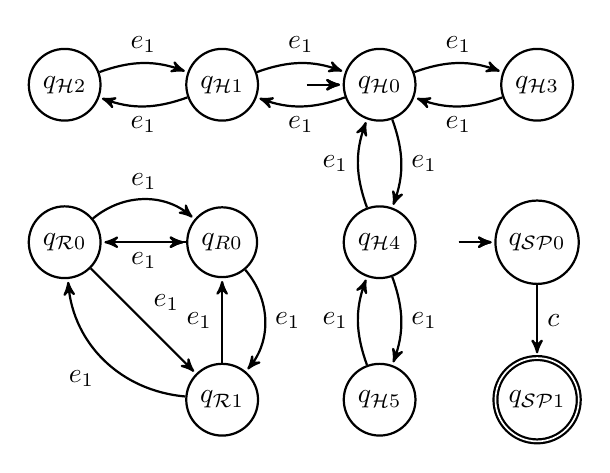
\begin{tikzpicture}[automatonFig]
		    %HUMAN
			\node [state, initial, initial] (qH1) at (4,0)     {$q_{\mathcal{H}0}$};
			\node [state] (qH2) at (2,0)     {$q_{\mathcal{H}1}$};
			\node [state] (qH3) at (0,0)     {$q_{\mathcal{H}2}$};
			\node [state] (qH4) at (6,0)     {$q_{\mathcal{H}3}$};
			\node [state] (qH5) at (4,-2)     {$q_{\mathcal{H}4}$};
			\node [state] (qH6) at (4,-4)     {$q_{\mathcal{H}5}$};			%ROBOT
        	\node [state, initial, initial] (qR0) at (2,-2)     {$q_{R0}$};
			\node [state] (qR1) at (0,-2)     {$q_{\mathcal{R}0}$};
			\node [state] (qR2) at (2,-4)     {$q_{\mathcal{R}1}$};
			%SPEC
			\node [state, initial, initial] (qS1) at (6,-2)     {$q_{\mathcal{SP}0}$};
			\node [state,accepting] (qS2) at (6,-4)     {$q_{\mathcal{SP}1}$};
			
			%			
			\path[->]
            %HUMAN
            (qH1) edge [bend left=20] node {$e_1$} (qH2)
			(qH2) edge [bend left=20] node {$e_1$} (qH1)
			
			(qH2) edge [bend left=20] node {$e_1$} (qH3)
			(qH3) edge [bend left=20] node {$e_1$} (qH2)
			
			(qH1) edge [bend left=20] node {$e_1$} (qH4)
			(qH4) edge [bend left=20] node {$e_1$} (qH1)
			
			(qH1) edge [bend left=20] node {$e_1$} (qH5)
			(qH5) edge [bend left=20] node {$e_1$} (qH1)
			
			(qH5) edge [bend left=20] node {$e_1$} (qH6)
			(qH6) edge [bend left=20] node {$e_1$} (qH5)
            
            %ROBOT
			(qR0) edge [bend left=0] node {$e_1$} (qR1)
			(qR1) edge [bend left=40] node {$e_1$} (qR0)
			
			(qR1) edge [bend left=0] node {$e_1$} (qR2)
			(qR2) edge [bend left=40] node {$e_1$} (qR1)
			
			(qR0) edge [bend left=40] node {$e_1$} (qR2)
			(qR2) edge [bend left=0] node {$e_1$} (qR0)
			
			%SPEC
			(qS1) edge node {$c$} (qS2)
            
			;
		    	
           
		\end{tikzpicture}\\
		
		\caption{EFSA models $\mathcal{H}$ (center), $\mathcal{R}$ (lower left), and safety spec $\mathcal{SP}$ (lower right).}
		\label{fig:EFSA_models}
	\end{figure}

\begin{table*}[]
    \centering
    \begin{tabular}{llll}
         \hline
         Event & Explanation & Guard & Action \\
         \hline
         $t_1$ & Transition between center and storage & - & -\\
         $t_2$ & Transition between center and robot & - & - \\
         $u_S$ & Pick up part from storage & \texttt{part\_status == 0} & \texttt{part\_status = 1} \\
         $d_S$ & Put down part at storage & \texttt{part\_status == 1} & \texttt{part\_status = 0}\\
         $u_R$ & Pick up part from robot& \texttt{part\_status == 2} & \texttt{part\_status = 1}; \texttt{collab\_space\_occ=1}\\
         $d_R$ & Put down part at robot& \texttt{part\_status == 0} & \texttt{part\_status = 2}; \texttt{collab\_space\_occ=1}\\
         $b_1$ & Press start button & \texttt{part\_status != 1}& \\
         $b_2$ & Press safety override button& \texttt{part\_status != 1} & \\
         $b_3$ & Press stop button & \texttt{part\_status != 1} & \\
         $r$   & Retract hands & - & - \\
         \hline
    \end{tabular}
    \caption{Caption}
    \label{tab:states_actions}
\end{table*}

Supervisor synthesis is also performed in supremica, which provides automated functionality for this task [verweis!].


\subsubsection{Simulation}
Simulations are performed in \textit{CoppeliaSim} simulator. An image of the simulation scene is shown in Fig. x. For the human model, we use CoppeliaSim's default human model \textit{Bill}. In order to model the inherent variability of human motion, several parameters human motion are randomized in the simulator (see Table x).

Since the safety specification $\mathcal{SP}$ only makes a binary safety decision, an additional metric is evaluated which quantifies the level of danger that is associated with a given human-robot configuration in a continuous value $r$.
\begin{equation}
	r = \begin{cases} 0 & \text{case (a):}\ v_R < v_{crit} \\
		\text{e}^{-d_{HR}} & \text{case (b):}\ v_R \geq  v_{crit};\ d_{HR}>0\\
		\frac{F_{\mathrm{c}}}{F_{\mathrm{max}}}+1 & \text{case (c):}\ v_R \geq  v_{crit};\ d_{HR}=0
	\end{cases}
	\label{eq:RiskMetric}
\end{equation}
After the analysis, this metric allows the user to spot hazardous situations without needing to inspect each simulation run individually.

\subsection{Comparison to other Methods}

\subsection{Results}

\section{DISCUSSION}
\label{sec:discussion}
\subsection{Reliability}
- Different Lvls. of Abstraction and their implications; True/False Positives/Negatives; Overapproximate safety criteria
- Modeling Effort, Modeling Bias
- Synthesis vs. Search-based Testing; Degree of required knowledge (black box, white box).
- Assumptions and their limitations
- Level of detail, human model
\subsection{}

\section{SUMMARY AND FUTURE WORK}
% This can be challenging, especially since human behavior is inherently non-deterministic and the possibility of human errors or other unforeseen behaviors must be considered, leading to a vast range of possible interaction scenarios that need to be analyzed. In recent years, two main approaches for the safety analysis of human-robot systems have emerged: Formal verification and Simulation-based testing. While both approaches have been discussed extensively in related work, literature on comparing and combining them is relatively rare.

% The contributions of this paper are twofold: First, we discuss the comparative advantages and disadvantages of formal verification and simulation-based testing. To illustrate this discussion, three different exemplary HRC scenarios from the industrial domain are modeled and analyzed using both formal verification and simulation.
% Second, we propose a novel approach which builds on the models from the aforementioned comparative study. We show how to systematically link formal verification and simulation using supervisory control theory. The proposed method is evaluated and discussed using the same example scenarios as mentioned above.

% \section{METHODS FOR ANALYZING HRC SYSTEMS}
% \label{sec:related_work}

% \subsection{Human Reasoning}
% ISO 12100 - Expert knoweldge - experience - intuitive tehcniques (e.g. brainstorming) - human reasoning supported by simple tools such as cehcklists or more sophisticated models (e.g. STPA w/ control structure diagram or HAZOP-UML w/ UML models).
% \subsection{Formal verification}
% Formal description of system behavior (often automata models) and formal specification of desired and/or undesired behaviors (often in LTL or also as automaton). Exhaustive exploration of all possible system states results in counterexample or formal proof of correct behavior (although in some cases no exhaustive exploration is possible, e.g. statistical model checking. Not considered further here).

% Examples: SAFER-HRC, Rathmair, ... others? --> see related work chapter in phd thesis.

% \subsection{Simulation-based testing}


% \subection{Advantages and Disadvantages}

% \section{CASE STUDY}
% \label{sec:comparison}

% \subsection{Approach}
% In this section, a case study is presented in which three different HRC scenarios from the industrial domain are modeled and analyzed using formal verification and simulation, respectively. As shown in section \ref{sec:related_work}, there are different methods for both formal verification and simulation-based analysis. In addition, for each method there are further use case specific considerations such as the choice of simulation tool or level of abstraction. It should therefore be emphasized that this comparative study is not intended to be representative of all types of formal verification and simulation methods. Rather, it is intended to identify and illustrate, in qualitative terms, common advantages, disadvantages, and problems. As an examplary formal verification tool, we choose \textit{Supremica}

% \subsection{Scenario Description}
% For brevity, only one of the three scenarios is presented in detail here. The remaining scenarios are available online\footnote{insert github link here}, with each scenario including the respective simulation and automata models as well as code and documentation.

% Fig x. shows the example scenario, consisting of a human worker, a robot, and a storage table. The worker can perform a set of actions, which are given by the following action space $A$:
% \begin{equation}
%     A=\{...\}
%     \label{eq:human_action_space}
% \end{equation}



% \subsection{Analysis with Formal Verification}

% \subsection{Simulation-based Analysis}

% \subsection{Comparison}

% \subsubsection{Qualitative}

% \subsubsection{Quantitative}

% \section{COMBINED APPROACH}
% \label{sec:combined_approach}

% \subsection{Preliminaries}

% \subsection{Approach}

% \subsection{Implementation and Testing}

% \section{DISCUSSION}
% \label{sec:discussion}

% \section{SUMMARY AND FUTURE WORK}
% \label{sec:summary_and_future_work}

% Note that the MDP-Automaton product need not to be built explicitly, but can be generated \emph{on-the-fly} when simulating the MDP. An optimal policy for any MDP extended by automata specifications can then be synthesized by applying an RL-algorithm to the \textit{product MDP}. In this paper, we utilize an approximate Q-learning method with linear function approximators and target Q-function $Q_\vartheta$ inspired by DDQN \cite{van2016deep} and detailed in Alg.~\ref{alg:Q-Learning}. If the RL algorithm only receives rewards from the automaton specification (i.e. $\varphi$), it can be proven that if there exists a policy such that the specification can be satisfied with probability one, the Q-learning will find such a policy \cite{sadigh2014learning,hasanbeig2019reinforcement}. 

% % \begin{algorithm}
% %     \caption{\small{Automaton Constrained Approximate Q-Learning}}
% %     \begin{algorithmic}
% %         \REQUIRE \small{Q-function parameters $\theta_i^a$ and $\vartheta_i^a$, replay memory $D$, automaton specification $\mathcal{SP}$ 
% %         \FORALL{episodes}
% %             \STATE Initialize $s$ and $q$
% %             \FORALL{steps of episode}
% %                 \STATE Choose $a$ $\epsilon$-greedily from $s$ using policy derived from $Q$
% %                 \STATE Take action $a$, observe $r$ and $s'$ 
% %                 \STATE Observe $\lambda$ and $q'$ of $\mathcal{SP}$
% %                 \STATE $r \leftarrow r + \lambda$
% %                 \STATE Store $((s, q), a, r, (s', q'))$ in $D$
% %                 \FORALL{$((s, q), a, r, (s', q'))$ in minibatch of $D$}
% %                     \FORALL{$\theta_i^a$}
% %                         \STATE $\theta_i^a \leftarrow \theta_i^a + \alpha \left[r + \gamma \max_{a} Q_\vartheta((s', q'), a) - Q_\theta((s, q),a) \right]f((s, q))$
% %                     \ENDFOR
% %                 \ENDFOR
% %                 \STATE Update target parameters $\vartheta_i^a \leftarrow 0.9 \cdot \vartheta_i^a + 0.1 \cdot \theta_i^a$ 
% %                 \STATE $s \leftarrow s'$
% %                 \STATE $q \leftarrow q'$
% %             \ENDFOR
% %         \ENDFOR 
% %         \RETURN $\pi^*(s) = \argmax_a Q(s,a)$}
% %     \end{algorithmic}
% %     \label{alg:Q-Learning}
% % \end{algorithm}

% % \begin{figure}
% %     \centering
% %     \subfloat{
% %         \begin{tikzpicture}[automatonFig,node distance=2.4cm]
% %               \node [state, initial, initial text={$G_1$}] (A) at (0,1)     {$s_1$};
% %               \node [state]                                         (B) [below right of=A] {$s_3$};
% %               \node [state]                                         (C) [above right of=B] {$s_2$};
            
% %               \path[->]
% %                 (A) edge node [font=\small] {$b,-0.1$} (B)
% %                 (A) edge node [font=\small] {$c,-0.25$} (C)
% %                 (A) edge [loop below] node [font=\small] {$a,0$} ()
% %                 (B) edge [bend right] node [font=\small]  {$c,-0.1$} (C)
% %                 ;
% %         \end{tikzpicture}}
% %     \hfil
% %     \subfloat{
% %         \begin{tikzpicture}[automatonFig,node distance=1.7cm]
% %               \node [state, initial, initial text={$SP_1$}] (X) at (0,1)     {$q_1$};
% %               \node [state, accepting] (Y) [below of=X] {$q_2$};;
            
% %               \path[->]
% %                 (X) edge node [font=\small] {$c,\lambda_{sp}$} (Y)
% %                 ;
% %         \end{tikzpicture}}
% %     \caption{An illustrative example for the effect of different reward magnitudes $\lambda_{sp}$ for satisfying a specification $SP_1$ on the optimal policy in system $G_1$. The double circle at $q_2$ indicate the state as marked (goal) state.}
% %     \label{fig:toy_system}
% % \end{figure}


% % \begin{algorithm}
% %     \caption{\small{DUAL SPSA}}
% %     \begin{algorithmic}
% %         \REQUIRE \small{Gradient step length parameters $A, B, \beta$, and perturbation coefficients $d, \kappa$
% %         \FORALL{steps $n$ in $[1, N]$}
% %             \STATE Compute gradient step length $\mu \leftarrow A/(B+n)^\beta$
% %             \STATE Compute perturbation magnitude $d_n \leftarrow d/n^\kappa$
% %             \STATE Sample $\Delta$ from a symmetric Bernoulli distribution 
% %             \STATE $\lambda^+ \leftarrow \lfloor \lambda + d_n \Delta \rfloor_0$
% %             \STATE $\lambda^- \leftarrow \lfloor\lambda - d_n \Delta \rfloor_0$
% %             \STATE Eval. dual problem at $h^+ = h(\lambda^+)$ by Q-learning (Alg. \ref{alg:Q-Learning})
% %             \STATE Eval. dual problem at $h^- = h(\lambda^-)$ by Q-learning (Alg. \ref{alg:Q-Learning})
% %             \STATE Estimate gradient of dual problem $\hat{\nabla} h = \frac{h^+ - h^-}{2 d_n \Delta}$
% %             \STATE Update automata rewards $\lambda \leftarrow \lambda - \textit{clip}(\mu \hat{\nabla}h, \underline{\mu \hat{\nabla}h}, \overline{\mu \hat{\nabla}h})$
% %         \ENDFOR
% %         \RETURN $\lambda$}
% %     \end{algorithmic}
% %     \label{alg:dual SPSA}
% % \end{algorithm}


% \section{FUTURE WORK}
% While the presented use-case study has clearly indicated the benefits of the newly proposed method, the SUT in this case had relatively weak safety measures, meaning that even the unsophisticated random sampling found a considerable amount of hazardous situations. It would be interesting to compare the approaches in test scenarios with stronger safety measures, where unsafe situations are more rare.

% Another issue to consider is that safety analyses are typically performed iteratively, meaning that after a hazardous situation is found, new safety measures are introduced and the search is then repeated on a slightly modified SUT. Investigating how different algorithms cope with such modifications is also a possible area for future research.

% Finally, it should be noted that this paper is focused primarily on conceptional aspects, and not necessarily on performance optimization of the algorithms themselves. Thus, further performance improvements are also under consideration for future work.





%%%%%%%%%%%%%%%%%%%%%%%%%%%%%%%%%%%%%%%%%%%%%%%%%%%%%%%%%%%%%%%%%%%%%%%%%%%%%%%%



%%%%%%%%%%%%%%%%%%%%%%%%%%%%%%%%%%%%%%%%%%%%%%%%%%%%%%%%%%%%%%%%%%%%%%%%%%%%%%%%
% \section*{APPENDIX}

% Appendixes should appear before the acknowledgment.

\section*{ACKNOWLEDGMENT}
The authors thank Tamim Asfour for his support.



%%%%%%%%%%%%%%%%%%%%%%%%%%%%%%%%%%%%%%%%%%%%%%%%%%%%%%%%%%%%%%%%%%%%%%%%%%%%%%%%





\bibliography{references.bib}
\bibliographystyle{IEEEtran}
\end{document}
